\documentclass[11pt,a4paper]{article}

\usepackage{../../templates/style}

\begin{document}

\begin{problem}{Magic Square}{standard input}{standard output}{1 second}{64 megabytes}

จตุรัสกลเป็นตารางขนาด $n \times n$ ที่ระบุจำนวนเต็มมีค่าตั้งแต่ $1$ ถึง $n^2$ เอาไว้ตามช่องต่าง ๆ ช่องละหนึ่งจำนวน โดยที่ผลรวมของตัวเลขในแนวนอน แนวตั้ง และแนวทแยงจะได้จำนวนเท่ากันเสมอ ตัวอย่างเช่น

\begin{figure}[h]
\centering
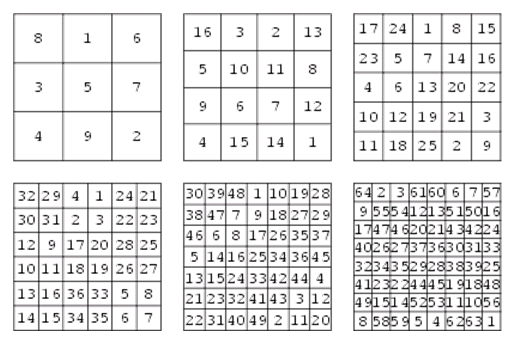
\includegraphics[width=0.7\textwidth]{../latex/img/1017/1017-1.png}
\end{figure}

\textbf{หมายเหตุ}: จตุรัสกลที่กล่าวถึงในโจทย์ข้อนี้ จะหมายถึง จตุรัสกลทั่วไป \textit{(Normal magic square)} ซึ่งจำนวนในแต่ละช่องจะต้องไม่ซ้ำกัน
\bigskip

\underline{\textbf{โจทย์}} จงเขียนโปรแกรมเพื่อตรวจสอบว่าตารางที่ให้มาเป็นจตุรัสกลหรือไม่

\InputFile

\textbf{บรรทัดแรก} เป็นจำนวนเต็ม $n$ $(1 \leq n \leq 10)$ ใช้กำหนดขนาดของตาราง
\textbf{บรรทัดที่ $2$ ถึง $n+1$} บรรทัดที่ $i+1$ รับข้อมูลของตารางในแถวที่ $i$ แต่ละบรรทัดเป็นจำนวนเต็ม $n$ จำนวนซึ่งคั่นด้วยช่องว่างหนึ่งช่อง โดยแต่ละค่ามีค่าอยู่ระหว่าง $1$ ถึง $n^2$

\OutputFile

\textbf{มีบรรทัดเดียว} พิมพ์คำว่า “Yes” ถ้าหากตารางที่ให้มาเป็นจตุรัสกล ไม่เช่นนั้นให้พิมพ์คำว่า “No” โดยไม่มีเครื่องหมายคำพูด

\Examples

\begin{example}
\exmp{4
16 2 3 13
5 11 10 8
9 7 6 12
4 14 15 1}{Yes}%
\end{example}


\Source

การแข่งขันคณิตศาสตร์ วิทยาศาสตร์ โอลิมปิกแห่งประเทศไทย สาขาวิชาคอมพิวเตอร์ ประจำปี 2547

\end{problem}

\end{document}